\documentclass[xcolor=dvipsnames, aspectratio = 169]{standalone}
%\usepackage[dvipsnames]{xcolor}
\usepackage{tikz}
\usetikzlibrary{shapes.geometric, arrows}


\tikzstyle{box1} = [rectangle, rounded corners, minimum width=3cm, minimum height=1.5cm,text centered, text width=3cm, draw=BlueGreen, fill=BlueGreen!40]

\tikzstyle{box2} = [rectangle, rounded corners, minimum width=3cm, minimum height=1.5cm,text centered, text width=3cm, draw=Thistle, fill=Thistle!40]

\tikzstyle{box3} = [rectangle, rounded corners, minimum width=3cm, minimum height=1.5cm,text centered, text width=3cm, draw=YellowGreen, fill=YellowGreen!40]

% \tikzstyle{box} = [rectangle, rounded corners, minimum width=3cm, minimum height=2cm,text centered, draw=BlueGreen, fill=BlueGreen!40]

\tikzstyle{arrow} = [ultra thick, BrickRed,->,>=stealth]

\begin{document}


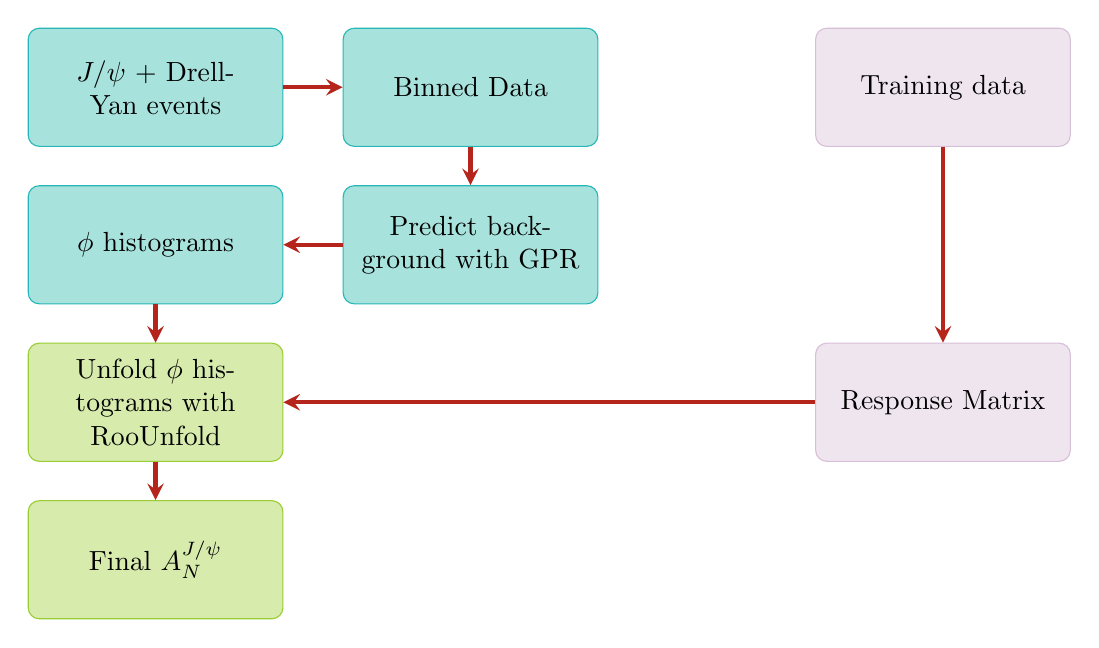
\begin{tikzpicture}[node distance=2cm]
\node (a0) [box1] {$J/\psi$ + Drell-Yan events};
\node (a1) [box1, right of=a0, xshift=2cm] {Binned Data};
\node (a2) [box1, below of=a1] {Predict background with GPR};
\node (a3) [box1, left of=a2, xshift=-2cm] {$\phi$ histograms};
%%%%%%
\node (a4) [box2, right of=a0, xshift=8cm] {Training data};
\node (a5) [box2, below of=a4, yshift=-2.0cm] {Response Matrix};
\node (a6) [box3, below of=a3] {Unfold $\phi$ histograms with RooUnfold};
\node (a7) [box3, below of=a6] {Final $A_{N}^{J/\psi}$};
%% draw arrows
\draw [arrow] (a0) -- (a1);
\draw [arrow] (a1) -- (a2);
\draw [arrow] (a2) -- (a3);
\draw [arrow] (a4) -- (a5);
\draw [arrow] (a3) -- (a6);
\draw [arrow] (a5) -- (a6);
\draw [arrow] (a6) -- (a7);
\end{tikzpicture}

\end{document}